\hspace{1.5cm}Potassium ion channels are membrane proteins critically involved in the regulation of fundamental physiological processes such as cell volume, membrane potential, and hormone secretion. To allow for the tuning of these processes, the human genome contains 78 potassium channels. The small- and intermediate conductance calcium-activated potassium channels are a group of proteins within the overall potassium channel family that share a set of common features.

One of their main features is that they are considered calcium-activated channels because their gating mechanism, in which potassium flux is regulated by the opening and closing of the channel, is modulated by a calcium-sensing protein called calmodulin.

\begin{figure}[h]
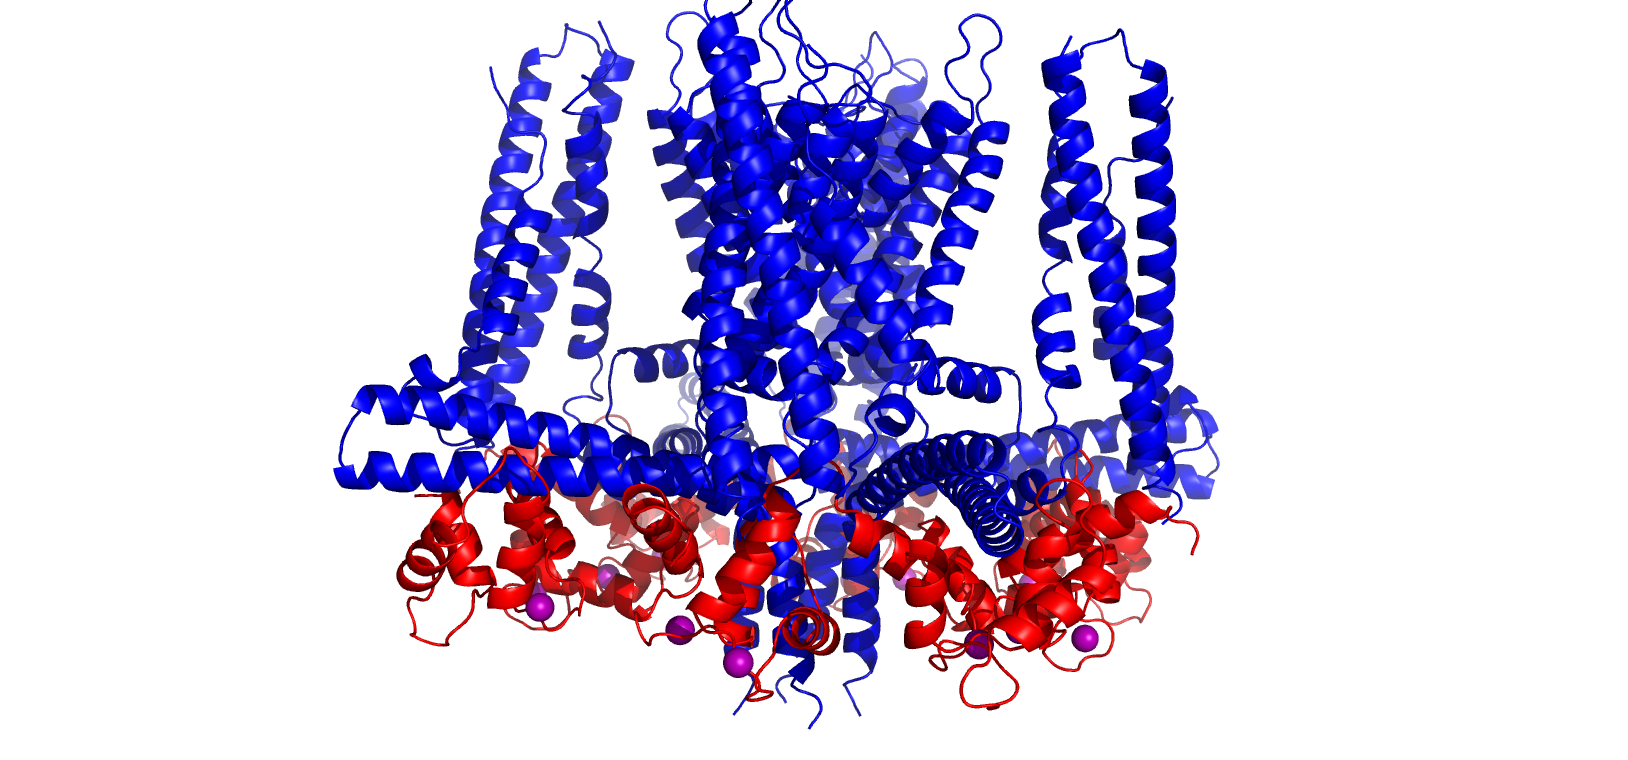
\includegraphics[width=15cm, height=7.5cm]{Images/Introduction/sk4.png}
\centering
\caption{Illustration of the $\text{K}_{\text{Ca}}3.1$ channel, based on the experimentally solved structure in \cite{sk4_struct}.}
\label{fig:Figure 3.1}
\end{figure}

In addition, small and intermediate conductance channels are so called because of their small single channel conductance in the order of 10 pS, in contrast with large conductance channels which have very high conductance in the range of 100 to 300 pS.

The protein studied in this study is the $\text{K}_{\text{Ca}}3.1$, and is a member of the small and intermediate conductance calcium-activated potassium channel subfamily, and is mainly expressed in red blood cells and cells of the immune system. Their structure, which was recently solved by MacKinnon \textit{et al.} \cite{sk4_struct} and is shown in Figure 1.1, is tetrameric, that is, it consists of four identical subunits. Each of these subunits contains six domains that insert into the cell membrane and form the potassium ion selectivity filter. In addition, the channel contains a calmodulin-binding domain inside the cell, where calcium-sensing calmodulin binds to the protein.  An schematic illustration of this structure is shown in Figure 1.2.

\begin{figure}[h]
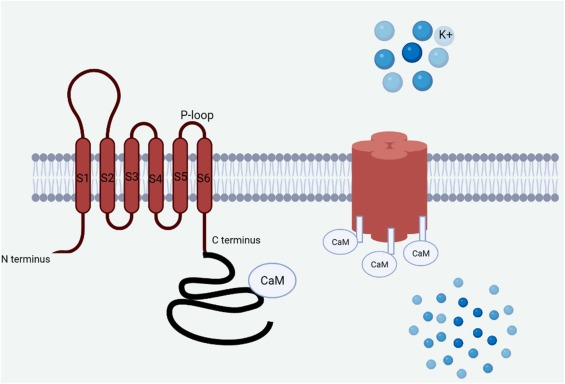
\includegraphics[width=12cm, height=7.5cm]{Images/Introduction/SK_Channel_schema.jpg}
\centering
\caption{General small and intermediate conductance channel structure. Four subunits form the channel complex (right). Each alpha subunit consists of 6 transmembrane domains (S1-S6) (left). Note N and C termini, with a calmodulin (CaM) binding domain at the C terminus of each subunit. Image from \cite{sk4_schema}.}
\label{fig:Figure 3.1}
\end{figure}

The main reason why this channel is interesting to us is that it has been validated as a potentially interesting pharmaceutical target. It has been shown that small molecule inhibitors of this channel may be used for the treatment of diseases such as vascular restenosis \cite{vascular_restenosis}, atherosclerosis \cite{atherosclerosis}, allograft vasculopathy \cite{allograft_vasculopathy}, inflammatory bowel disease \cite{inflammatory_bowel_disease}, ischemic stroke \cite{ischemic_stroke}, and renal \cite{renal_fibrosis} and cardiac fibrosis \cite{cardiac_fibrosis}. The action mechanism of one of these inhibitors is shown in Figure 1.3, where it can be seen that the inhibitor lies in the middle of the channel gate blocking the flow of potassium in and out of the channel and thus reducing its conductance.

Despite their potential application, no small molecule $\text{K}_{\text{Ca}}3.1$ channel inhibitors that are suitable for clinical use are known yet, due to different pharmacological issues with the currently known inhibitors. This serves as the main motivation for this work, where we are interested in analysing whether computation techniques based on machine learning can serve as useful aids in the search of clinically viable $\text{K}_{\text{Ca}}3.1$ channel inhibitors.

\begin{figure}[h]
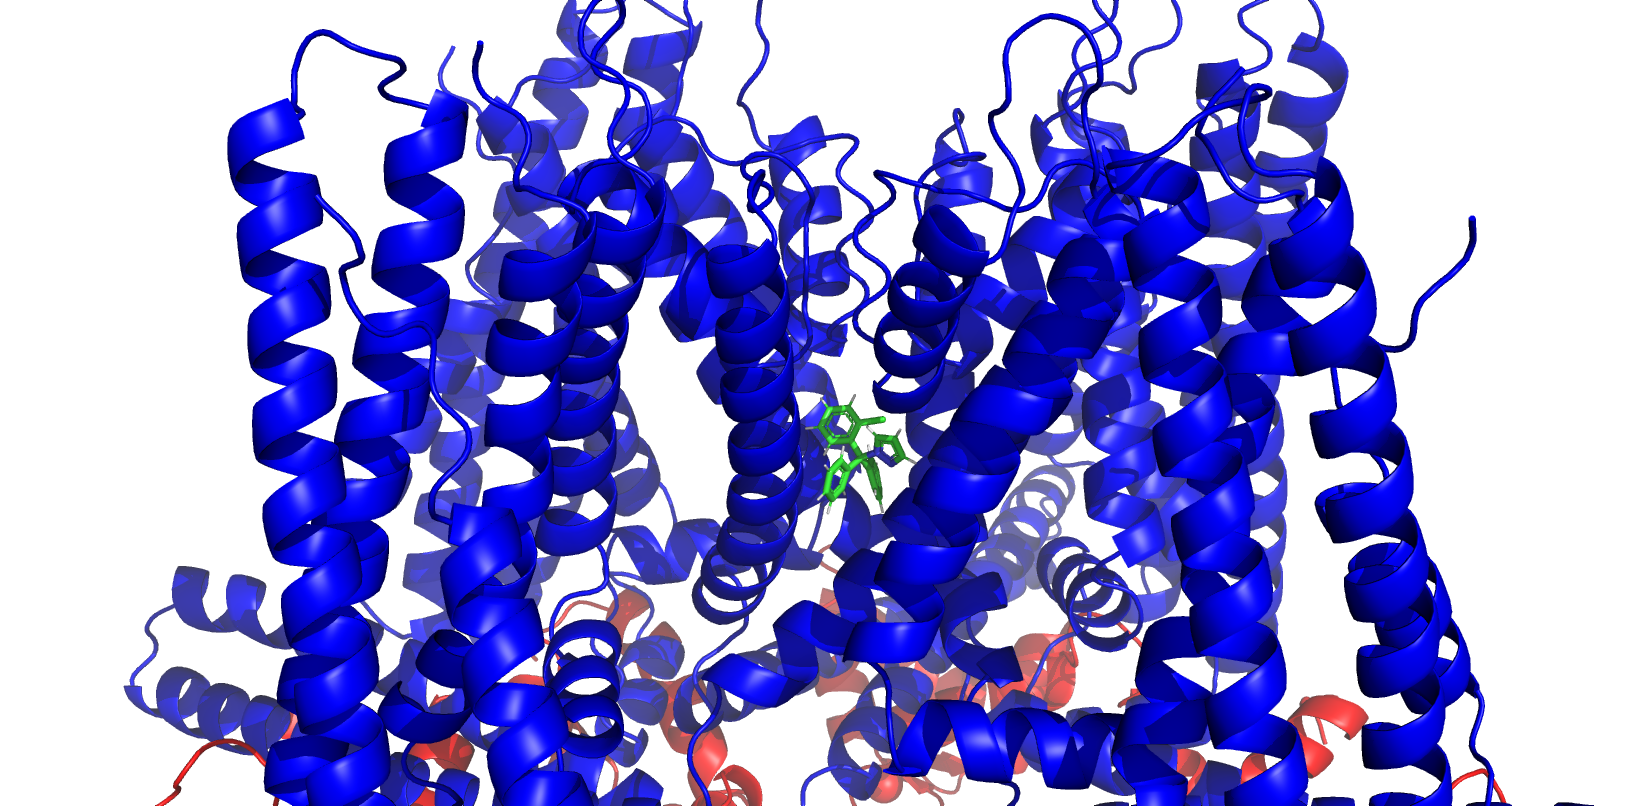
\includegraphics[width=12cm, height=7.5cm]{Images/Introduction/tram34_docking.png}
\centering
\caption{Bound conformation of the TRAM-34 ligand in the binding pocket of the $\text{K}_{\text{Ca}}3.1$ channel that lies at its gate. TRAM-34 is a distinguished and potent inhibitor of intermediate conductance in calcium-activated potassium channels.}
\label{fig:Figure 3.1}
\end{figure}

In recent years, as traditional experimental techniques for the discovery of new drugs have gradually become more expensive and less effective, computational techniques have become significantly more relevant in the field of drug development.

One of the most common computational techniques for drug development is molecular docking, which is used to predict the binding of small molecules (also referred to as ligands in this context) to a target protein of interest (also referred to as a receptor in this context). While these techniques have become quite accurate in predicting the geometric conformations that these ligands adopt when binding to most systems, they are much less effective in predicting the binding affinity between the ligands and the receptor. The binding affinity indicates how favourable the binding is between the ligand and the receptor, and can be understood as the difference in free energy between the bound and unbound systems.

This measure is extremely important for drug discovery because it can be used to distinguish nonbinding ligands and to identify binders in large compound libraries with a very large number of molecules. It is also used in the context of lead optimisation, where the goal is usually to identify the most effective molecules among those that have a similar chemical structure to a lead.

To predict this binding affinity, docking algorithms use $scoring$ $functions$ with a predetermined functional form inspired by theory for the relationship between the features that characterize the protein-ligand complex and its predicted binding affinity. It is almost always assumed that this relationship is linear. However, many complexes do not conform to this strong modeling assumption, and in these cases less accurate predictions are obtained.

Because of these limitations, there has been recent interest in using data-driven machine learning strategies to predict binding affinities between ligands and receptors. Machine learning algorithms are able to circumvent the constraint of a fixed functional form for the scoring function and can therefore implicitly capture intermolecular binding interactions that are difficult to model explicitly.\\

With this in mind, the main goal of this work is to investigate whether we are able to use machine learning strategies to improve the performance of conventional scoring functions, and thus serve as a potential contribution to future studies aimed at finding inhibitors that are clinically useful. Therefore, our strategy will be to use the docking simulations to predict the binding conformation of the inhibitors of the $\text{K}_{\text{Ca}}3.1$ channel, and then based on features of this conformation, along with features inherent to the chemical structure of the ligands, develop an algorithm that accurately predicts the binding affinity between the ligand and the receptor.